\documentclass[a4paper,fleqn]{cas-sc}

\usepackage[numbers]{natbib}


\usepackage{amssymb}
\usepackage{amsmath}
\usepackage{array}
\usepackage{colortbl}   
\usepackage{booktabs} 
\usepackage{xcolor}   
\usepackage{caption}
\usepackage{adjustbox}
\usepackage{float}
\usepackage{subcaption}
\usepackage{graphicx}
\usepackage{placeins}
\usepackage{enumitem}
\usepackage{xparse}
\usepackage{expl3}
\usepackage{algorithm}
\usepackage{algpseudocode}
\usepackage{caption}
\captionsetup[table]{position=bottom}
\captionsetup[table]{justification=centering, position=bottom}

\usepackage{tikz}
\usetikzlibrary{shapes.geometric, arrows, positioning, calc}
\tikzstyle{startstop} = [rectangle, rounded corners, minimum width=3cm, minimum height=1cm,text centered, draw=black, fill=red!30]
\tikzstyle{io} = [trapezium, trapezium left angle=70, trapezium right angle=110, minimum width=3cm, minimum height=1cm, text centered, draw=black, fill=blue!30]
\tikzstyle{process} = [rectangle, minimum width=3cm, minimum height=1cm, text centered, draw=black, fill=orange!30]
\tikzstyle{decision} = [diamond, minimum width=3cm, minimum height=1cm, text centered, draw=black, fill=green!30]
\tikzstyle{arrow} = [thick,->,>=stealth]




\begin{document}
\captionsetup{justification=centering}
\let\WriteBookmarks\relax
\def\floatpagepagefraction{1}
\def\textpagefraction{.001}
\shorttitle{Physics-Guided Unsupervised Latent Alignment for Unified Solar PV System Loss Estimation}

\title [mode = title]{Physics-Guided Unsupervised Latent Alignment for Unified Solar PV System Loss Estimation}                      

\author[1]{Aruni Saxena}
\ead{202418006@dau.ac.in}
\credit{Conceptualization, Methodology, Software, Writing - Original Draft}

\author[1]{Arpit Rana}
\cormark[1]
\ead{arpit_rana@dau.ac.in}
\credit{Supervision, Project administration, Writing - Reviewing \& Editing}

\author[1]{Sreeja Rajendran}
\ead{sreeja_rajendran@dau.ac.in}
\credit{Validation, Investigation}

\affiliation[1]{organization={Dhirubhai Ambani University},
                city={Gandhinagar},
                postcode={382007}, 
                state={Gujarat},
                country={India}}

\cortext[cor1]{Corresponding author}

\begin{highlights}
\item Introduces a physics-informed unsupervised framework for latent solar PV loss estimation.
\item Aligns multiple modeling frameworks for a baseline consensus of system losses.
\item Incorporates explicit environmental physics for dust, rainfall, and humidity.
\item Evaluates statistical significance of physics-informed corrections across climates.
\item Validates results using national-level statistics and system-level SCADA data.
\end{highlights}


\begin{abstract}
The quantification of photovoltaic (PV) system losses under non-idealized, real-world operating conditions remains a fundamental challenge for energy meteorology and asset management. Conventional performance frameworks—while computationally robust for system sizing—routinely fail to capture the complex, non-stationary interplay between environmental forcing and system degradation, leading to systematic uncertainties in energy yield assessment. This paper reformulates PV loss estimation as a latent inference problem under incomplete observability.

We propose a physics-informed representation learning framework that treats PV system loss as an unobserved latent state. By aligning divergent outputs from established simulation models (PVWatts, SAPM, CEC, SAM) within a shared embedding, we extract a consensus latent baseline that reflects current modeling practice. We then enrich this baseline by embedding explicit physical mechanisms—including dust mass balances, rainfall cleaning kinetics, humidity-driven degradation, and coastal aerosol effects—into the representation architecture.

Through non-parametric hypothesis testing across climatic regimes in India, we show that physics-informed latent models reveal systematic discrepancies in conventional frameworks, particularly regarding seasonal memory effects. Validation against SCADA data from a single installation suggests that the framework captures seasonal dynamics that static derating models overlook. While the approach shows promise, generalization requires multi-site validation. This work contributes a methodological framework for physics-informed PV loss estimation that may inform future research on environmental performance diagnostics.
\end{abstract}



\begin{keywords}
photovoltaic system losses \sep
physics-informed machine learning \sep
latent variable modeling \sep
environmental degradation \sep
solar energy performance \sep
payback analysis
\end{keywords}

\maketitle



\section{Introduction}

The global transition to solar photovoltaics (PV) as a primary energy source has necessitated advances in performance diagnostics beyond high-level energy yield projection. However, a persistent challenge remains: the inability to directly measure environmental losses of field-deployed systems. While laboratory conditions permit isolation of loss mechanisms, real-world installations are subjected to coupled environmental stressors—soiling, thermal stress, humidity exposure, and spectral shifts—that are only observable through their aggregate effect on power output.

Traditionally, this challenge has been addressed through standardized performance frameworks, notably PVWatts~\cite{pvwatts}, the Sandia Array Performance Model (SAPM)~\cite{king2004sandia}, the California Energy Commission (CEC) model~\cite{cec_model}, and the System Advisor Model (SAM)~\cite{sam_nrel}. These frameworks have enabled large-scale solar deployment by providing consistent methods for system designers. However, these models rely on static derate factors or simplified empirical coefficients that assume temporal stationarity—an assumption that may not hold under seasonal dust accumulation, rainfall-driven recovery, and climate-dependent degradation.

In this context, we propose treating PV system loss as a latent variable—a quantity that cannot be directly measured but may be inferred from multiple model outputs. The estimates produced by conventional models are interpreted not as competing truths, but as imperfect observations of an underlying loss process. This perspective shifts the objective from forward simulation to joint inference constrained by environmental physics.

This paper presents a physics-informed latent alignment approach. Rather than replacing existing PV models, we synchronize their outputs within a shared latent space using an encoder--decoder architecture. We then refine this consensus by embedding explicit physical models of environmental forcing—including soiling deposition kinetics and humidity-driven degradation—into the representation learning process.

By applying this framework to diverse climatic sites across the Indian subcontinent, we address three critical research questions:
(i) How much "hidden uncertainty" exists between established PV modeling frameworks when subjected to real-world climatic variability?
(ii) Can explicit environmental physics recover the seasonal "memory effects" that are systematically omitted by traditional derating methods?
(iii) Is the divergence between baseline consensus and physics-informed inference statistically significant enough to alter the financial and policy outlook of solar projects?

The remainder of this paper is structured to reflect this narrative of discovery. Section 2 establishes the theoretical background and structural limitations of existing paradigms. Section 3 motivates the latent inference perspective through a lens of information theory and signal processing. Section 4 details our unified methodology, deriving the physics-based components from first principles and describing the latent alignment architecture. Section 5 presents the experimental design and statistical protocol, followed by a rigorous analysis of seasonal and spatial results in Section 6. We conclude in Section 7 by discussing the implications for the future of physics-informed PV intelligence~\cite{dipiazza2021artificial, karniadakis2021physics}.



\section{Background}

\subsection{Photovoltaic Performance Modeling and Loss Estimation}

Photovoltaic (PV) performance modeling has traditionally been developed to support 
system design, energy yield prediction, and techno-economic assessment under assumed 
operating conditions. Early modeling approaches focused on translating standard test 
condition (STC) ratings into expected field performance using simplified irradiance 
transposition and temperature correction formulations. Over time, several widely 
adopted modeling frameworks have emerged as de facto standards in both academic and 
industrial practice, including PVWatts~\cite{pvwatts}, the Sandia Array Performance 
Model (SAPM)~\cite{king2004sandia}, the California Energy Commission (CEC) model~\cite{cec_model}, 
and the System Advisor Model (SAM)~\cite{sam_nrel}.

These frameworks have played a critical role in enabling large-scale deployment of 
solar energy by providing computationally efficient and accessible estimates of 
system output. However, their primary objective is forward simulation of PV 
performance under assumed operating regimes rather than inference of underlying loss 
mechanisms from observed environmental variability. Consequently, losses are typically 
represented through aggregated derate factors or simplified empirical corrections, 
which limits their ability to capture site-specific and time-dependent degradation 
processes.

\subsection{Framework-Specific Assumptions and Structural Limitations}

PVWatts adopts a deliberately simplified modeling philosophy in which aggregate system 
losses are represented using fixed derate factors that account for soiling, wiring, 
mismatch, degradation, and availability~\cite{pvwatts}. While this approach enables 
Rapid assessment across diverse locations, it implicitly assumes temporal stationarity 
of loss processes and does not model environmental persistence, seasonal asymmetry, or 
recovery effects~\cite{sayyah2014yield, mani2010impact}. As a result, PVWatts loss estimates remain relatively insensitive to 
site-specific climatic dynamics such as prolonged dry periods or rainfall-driven 
natural cleaning~\cite{adams2015soiling, pavan2011effect}.

The Sandia Array Performance Model introduces greater electrical fidelity by explicitly 
modeling current--voltage behavior, spectral effects, and temperature dependence at the 
module level~\cite{king2004sandia}. Despite this increased physical detail, SAPM assumes 
optically clean and mechanically stable operating conditions. Environmental degradation 
mechanisms such as dust accumulation, humidity-induced optical losses, and corrosion 
are not explicitly represented, and their effects are absorbed indirectly into model 
calibration parameters~\cite{kimber2006effect, deceglie2018performance, hammock2012dust}.

The CEC model further refines electrical parameterization through standardized module 
coefficients derived from controlled laboratory measurements~\cite{cec_model}. Its 
formulation is well suited for comparative module evaluation and system sizing but 
remains largely agnostic to environmental processes beyond temperature effects. Optical 
soiling, long-term humidity exposure, and location-dependent degradation mechanisms 
are outside the scope of the model, constraining its applicability for long-term field 
performance analysis~\cite{pavan2011effect, adams2015soiling, gostein2013measuring}.

SAM integrates multiple modeling components, including irradiance transposition, 
thermal behavior, inverter performance, and financial analysis~\cite{sam_nrel}. While 
it allows users to specify environmental losses, these are typically implemented as 
static or user-defined derate inputs rather than dynamically evolving processes. As a 
result, SAM inherits many of the same structural limitations as other frameworks when 
applied to regions with strong seasonal cycles, heterogeneous aerosol loading, or 
climate-driven degradation trends.

\subsection{Loss Estimation as a Latent Inference Problem}

A common characteristic across existing PV performance frameworks is that system 
losses are not directly observable quantities within operational datasets. Field 
measurements typically provide aggregate power output, irradiance, and temperature, 
but do not isolate the contribution of individual loss mechanisms such as soiling, 
thermal stress, or humidity-induced degradation. As a result, framework-specific loss 
estimates represent indirect projections shaped by modeling assumptions rather than 
direct measurements of physical degradation processes.

This observation motivates treating PV system loss as a latent physical variable that 
must be inferred from multiple imperfect and biased observations. Differences among 
PVWatts, SAPM, the CEC model, and SAM should therefore be interpreted not as conflicting 
estimates of ground truth, but as reflections of distinct modeling abstractions and 
omitted physical processes. Without explicit representation of environmental memory, 
temporal persistence, and spatial heterogeneity, existing frameworks are structurally 
limited in their ability to infer true climate-induced loss trajectories.

\subsection{Need for Physics-Informed Latent Modeling}

Recent advances in physics-informed machine learning offer a principled pathway for 
addressing the limitations of static derate-based loss modeling. By combining 
physically motivated constraints with data-driven representation learning, it becomes 
possible to infer latent processes that are consistent with known environmental 
drivers while remaining robust to the absence of labeled loss data~\cite{raissi2019physics,karniadakis2021physics, li2022physics, huller2021physics}.

Rather than replacing existing PV performance frameworks, a physics-informed latent 
modeling approach can leverage them as informative but incomplete sensors of the 
underlying loss process. Aligning their outputs within a shared latent representation 
allows extraction of the consensus embedded in current modeling practice, while the 
explicit introduction of environmental physics enables systematic correction of shared 
omissions. This paradigm reframes PV loss estimation from deterministic simulation 
toward structured inference, enabling improved interpretability, reduced bias, and 
greater relevance for long-term performance assessment and policy analysis.


\section{Motivation}

Reliable estimation of photovoltaic (PV) system losses under real-world operating 
conditions is essential for energy yield prediction, financial modeling, and 
policy-driven deployment planning. However, system losses are not directly observable 
quantities in operational datasets. Measurements typically provide aggregate power 
output, irradiance, and temperature, but do not isolate the contributions of 
individual environmental and degradation mechanisms. This structural absence of 
labeled loss data fundamentally limits the applicability of supervised learning 
approaches and motivates a latent-variable perspective on PV loss estimation.

At the same time, PV system performance is routinely evaluated using multiple 
established simulation frameworks, each encoding distinct physical assumptions and 
abstractions. When applied to the same site and environmental conditions, these 
frameworks often produce substantially different loss estimates. Rather than 
interpreting these discrepancies as competing truths, this work is motivated by the 
view that each estimate represents a noisy and biased projection of a shared but 
unobserved physical quantity, namely the true climate-induced PV system loss.

From a statistical standpoint, PV loss estimation can therefore be formulated as an 
inference problem over an unobserved latent process. Existing performance models 
provide multiple imperfect observations of this process, each distorted by 
model-specific simplifications and omitted physical mechanisms. Simple averaging or 
regression-based reconciliation of these estimates is insufficient, as such 
approaches implicitly assume independent and unbiased observations and fail to 
account for temporal dependence, seasonal nonstationarity, and spatial heterogeneity.

A natural first step in this setting is to extract a consensus latent estimate from 
existing frameworks. However, consensus alone does not resolve shared bias. If all 
models omit the same environmental mechanisms—such as dust accumulation persistence, 
humidity-driven degradation memory, or rainfall-induced recovery—then agreement among 
their estimates remains systematically incomplete. This motivates the need for an 
explicit corrective mechanism rather than purely statistical alignment.

Environmental loss processes in PV systems exhibit structured dynamics that are 
poorly captured by static derate factors or instantaneous corrections. Soiling 
accumulates gradually over dry periods and is removed abruptly by rainfall, humidity 
induces degradation with long-term persistence, and thermal stress interacts 
nonlinearly with irradiance and seasonal climate regimes. These characteristics 
suggest that PV loss evolution is governed by temporally coupled and physically 
constrained processes rather than independent daily perturbations.

Physics-informed representation learning offers a principled pathway for embedding 
such structure within a latent inference framework~\cite{raissi2019physics,karniadakis2021physics, huller2021physics, wang2022physics}. 
By constraining latent representations using physically motivated formulations while 
retaining flexibility through data-driven learning, it becomes possible to infer loss 
trajectories that are both statistically consistent with observed model outputs and 
causally grounded in environmental drivers~\cite{liu2023physics, kim2023physics, hegde2022physics}.

Finally, meaningful correction of existing loss estimates should be empirically 
detectable. If explicit environmental physics materially alters inferred losses, this 
difference should manifest as a statistically significant divergence between baseline 
latent estimates derived from conventional frameworks and physics-informed latent 
losses. Conversely, the absence of such divergence would suggest that existing models 
already encode sufficient environmental information. This hypothesis-driven 
perspective motivates formal statistical evaluation of inferred latent loss processes 
in the absence of direct ground-truth measurements.

Collectively, these considerations motivate a unified framework that treats PV system 
loss estimation as a structured latent inference problem, integrates explicit 
environmental physics into representation learning, and evaluates outcomes through 
rigorous statistical testing rather than direct supervision.
.

\section{Methodology: Unified Environmental Physics--Informed Latent Loss Model}

This work formulates photovoltaic (PV) system loss estimation as a spatio-temporal 
latent inference problem under incomplete observability. The proposed methodology 
integrates site-specific environmental observations, physically motivated loss 
formulations, and unsupervised representation learning to infer a unified loss 
trajectory without imposing strong aggregation assumptions implicit in existing 
performance models.

\subsection{Limitations of Conventional Performance Frameworks}

Widely used PV performance frameworks such as PVWatts, SAPM, the CEC model, and SAM 
represent environmental losses using static derate factors or simplified empirical 
corrections~\cite{pvwatts,king2004sandia,cec_model,sam_nrel}. While these approaches 
are suitable for system sizing and forward simulation, they exhibit structural 
limitations when applied to long-term, site-specific loss estimation. In particular, 
they do not explicitly model time-dependent dust accumulation and rainfall-driven 
cleaning, humidity-induced degradation persistence, coastal corrosion effects, 
monsoon-specific irradiance suppression, or interannual climatic variability. These 
omissions motivate a unified formulation in which environmental physics are modeled 
explicitly and loss aggregation is inferred rather than assumed.

\subsection{Spatio-Temporal Environmental Data}

Environmental forcing variables are obtained from gridded datasets provided by the 
India Meteorological Department (IMD)~\cite{imd_data}. For each PV installation located at latitude 
$\lambda$ and longitude $\varphi$, environmental variables are spatially interpolated 
from surrounding grid points using Shepard's method~\cite{shepard1968two} and temporally aligned to construct site-specific daily 
trajectories:
\[
X_t(\lambda, \varphi) = \{AOD_t, R_t, RH_t, T_t, GHI_t\}.
\]
The physically-augmented conceptual model linking these atmospheric drivers to latent state evolution is illustrated in Figure~\ref{fig:physics}, following established modeling principles for desert and tropical environments~\cite{beattie2012sand, goossens2016wind, zorrilla2013soiling}.

\begin{figure}[htbp]
	\centering
	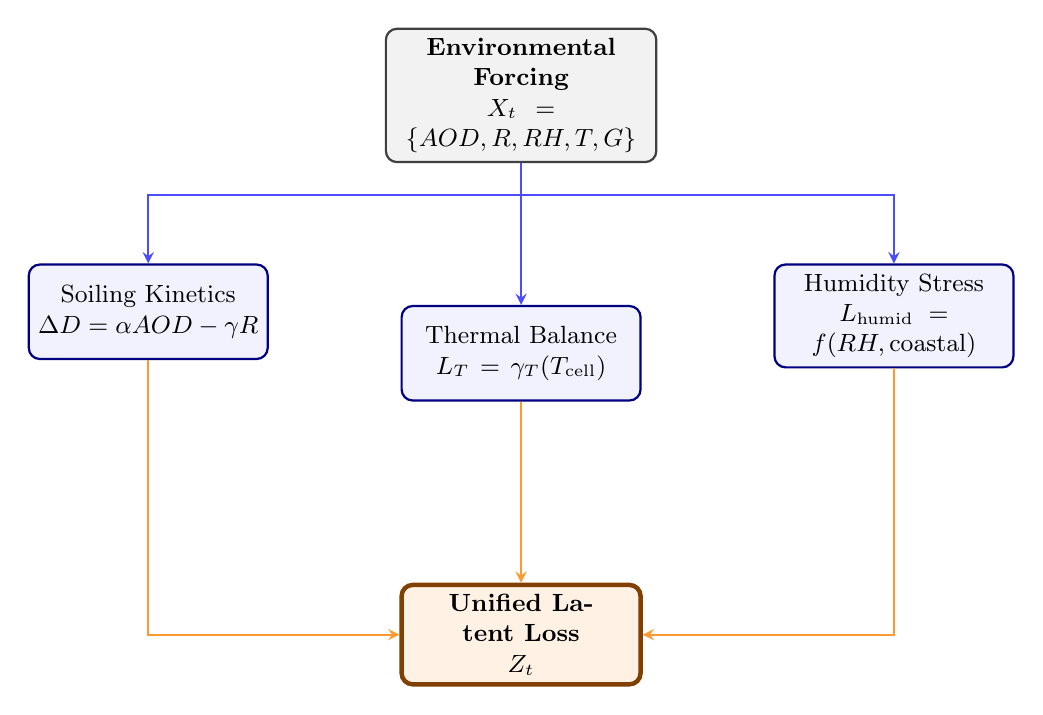
\begin{tikzpicture}[node distance=1.8cm, 
		box/.style={rectangle, draw=blue!50!black, fill=blue!5, text width=2.8cm, text centered, rounded corners, minimum height=1.2cm, thick, font=\small},
		input/.style={rectangle, draw=gray!50!black, fill=gray!10, text width=3.2cm, text centered, rounded corners, minimum height=1.2cm, thick, font=\small\bfseries},
		latent/.style={rectangle, draw=orange!50!black, fill=orange!10, text width=2.8cm, text centered, rounded corners, minimum height=1.2cm, ultra thick, font=\small\bfseries}]
		
		\node (input) [input] {Environmental Forcing \\ $X_t = \{AOD, R, RH, T, G\}$};
		\node (dust) [box, below left=of input, xshift=-0.2cm] {Soiling Kinetics \\ $\Delta D = \alpha AOD - \gamma R$};
		\node (humid) [box, below right=of input, xshift=0.2cm] {Humidity Stress \\ $L_{\text{humid}} = f(RH, \text{coastal})$};
		\node (thermal) [box, below=of input] {Thermal Balance \\ $L_T = \gamma_T(T_{\text{cell}})$};
		
		\draw[->, >=stealth, thick, blue!70] (input.south) -- ++(0,-0.4) -| (dust.north);
		\draw[->, >=stealth, thick, blue!70] (input.south) -- ++(0,-0.4) -| (humid.north);
		\draw[->, >=stealth, thick, blue!70] (input.south) -- (thermal.north);
		
		\node (loss) [latent, below=of thermal, yshift=-0.5cm] {Unified Latent Loss \\ $Z_t$};
		
		\draw[->, >=stealth, thick, orange!80] (dust.south) |- (loss.west);
		\draw[->, >=stealth, thick, orange!80] (humid.south) |- (loss.east);
		\draw[->, >=stealth, thick, orange!80] (thermal.south) -- (loss.north);
	\end{tikzpicture}
	\caption{Physically-augmented conceptual model of environmental loss mechanisms. The framework explicitly links atmospheric forcing to latent state evolution through derived kinetics of deposition and stress accumulation.}
	\label{fig:physics}
\end{figure}

Here, $AOD_t$ denotes an aerosol optical depth proxy, $R_t$ daily rainfall, $RH_t$ 
relative humidity, $T_t$ ambient temperature, and $GHI_t$ global horizontal 
irradiance. This formulation ensures that loss processes are driven by location- and 
time-resolved environmental conditions rather than climatological averages.

\subsection{Physics-Based Environmental Loss Components}

Environmental losses are modeled using physically motivated formulations designed to 
preserve temporal memory and nonlinear response.

\subsubsection*{Soiling and Dust Accumulation}

Dust accumulation is modeled as a discrete-time balance between aerosol deposition 
and rainfall-induced removal:
\[
D_{t+1} = D_t + \alpha AOD_t - \gamma R_t,
\]
where $D_t$ represents accumulated dust mass, $\alpha$ a deposition coefficient, and 
\]
where $k$ denotes an optical attenuation constant~\cite{bergin2017large, javed2016environmental, micheli2021change}.

\begin{figure}[H]
	\centering
	\includegraphics[width=0.95\textwidth]{physics_mechanisms_diagram_1770568736550.png}
	\caption{Environmental Forcing Schematic: Graphical representation of the embedded physical mechanisms. (A) Soiling kinetics following a discrete-time mass balance with rainfall-driven recovery. (B) Humidity-induced efficiency degradation modulated by coastal proximity. (C) Thermal derating pathways based on gridded IMD irradiance fields.}
	\label{fig:mechanisms}
\end{figure}

\subsubsection*{Humidity-Driven and Coastal Degradation}

Long-term degradation due to sustained humidity exposure is modeled as
\[
L_{\text{humid}} = 1 - \exp(-\beta f_{\text{humid}}),
\]
where $f_{\text{humid}}$ denotes the fraction of days with relative humidity exceeding 
a specified threshold and $\beta$ represents material susceptibility. To account for 
salt-induced corrosion in coastal environments, $\beta$ is spatially modulated as
\[
\beta_{\text{site}} = \beta \left(1 + \frac{C}{d + 1}\right),
\]
where $C$ denotes a salt aerosol concentration index and $d$ the distance from the 
coastline~\cite{toth2018soiling, soni2021assessment}.

\subsubsection*{Seasonal Clouding and Rainfall Cleaning}

Seasonal irradiance suppression during monsoon periods is modeled as
\[
L_{\text{cloud}}(t) = 1 - \frac{G_{\text{monsoon}}}{G_{\text{annual}}},
\]
where $G_{\text{monsoon}}$ and $G_{\text{annual}}$ denote mean monsoon-season and 
annual irradiance, respectively. Rainfall-driven cleaning is represented as a 
negative increment in soiling loss, capturing abrupt recovery events following heavy 
precipitation.

\subsubsection*{Temperature-Induced Losses}

Cell temperature is estimated using an irradiance-coupled NOCT formulation~\cite{fuentes1987simplified}:
\[
T_{\text{cell}} = T_{\text{amb}} + \frac{NOCT - 20}{800} G_t,
\]
and the corresponding temperature-induced power loss is computed as
\[
L_T(t) = \gamma_T (T_{\text{cell}} - 25),
\]
where $\gamma_T$ denotes the temperature coefficient of power~\cite{fuentes1987simplified, deceglie2018performance}.

\subsection{System-Level Loss Components}

In addition to environmental losses, system-level losses including wiring resistance, 
inverter inefficiency, module mismatch, and availability are incorporated as 
quasi-static components:
\[
L_{\text{sys}} = \{L_{\text{wire}}, L_{\text{inv}}, L_{\text{mismatch}}, L_{\text{avail}}\}.
\]
These terms ensure realistic total loss magnitudes while remaining independent of 
environmental dynamics.

\subsection{Latent Loss Inference via Unsupervised Representation Learning}

All environmental and system-level losses are assembled into an observed loss vector:
\[
Y_t = \{L_{\text{soil}}, L_{\text{humid}}, L_{\text{cloud}}, L_T, L_{\text{sys}}\}_t.
\]
This hierarchical inference architecture is visualized in Figures~\ref{fig:framework} and~\ref{fig:system_design}.
Rather than aggregating these components through a predefined functional form, an 
unsupervised encoder--decoder architecture is employed to infer a latent total loss:
\[
Z_t = \psi(Y_t; \phi),
\]
with a decoder
\[
\hat{Y}_t = h(Z_t; \theta).
\]
Model parameters are learned by minimizing reconstruction error:
\[
\mathcal{L} = \frac{1}{T} \sum_{t=1}^{T} \|Y_t - \hat{Y}_t\|_2^2.
\]

\begin{figure}[H]
	\centering
	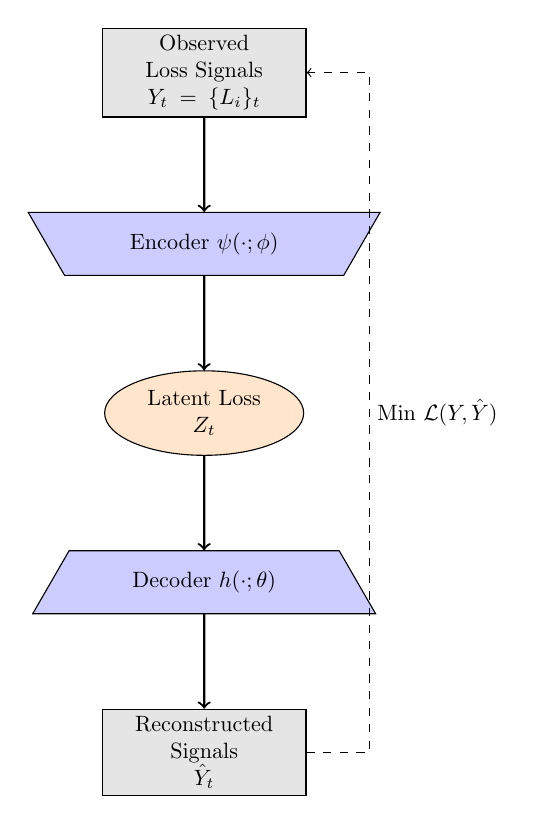
\begin{tikzpicture}[node distance=1.2cm, auto, scale=0.8, every node/.style={scale=0.8}]
		\node (obs) [rectangle, draw, fill=gray!20, text width=3cm, text centered, minimum height=1cm] {Observed Loss Signals \\ $Y_t = \{L_i\}_{t}$};
		\node (enc) [trapezium, draw, fill=blue!20, trapezium left angle=120, trapezium right angle=120, minimum width=2.5cm, minimum height=1cm, below=of obs] {Encoder $\psi(\cdot; \phi)$};
		\node (latent) [ellipse, draw, fill=orange!20, text width=2cm, text centered, minimum height=1cm, below=of enc] {Latent Loss \\ $Z_t$};
		\node (dec) [trapezium, draw, fill=blue!20, trapezium left angle=60, trapezium right angle=60, minimum width=2.5cm, minimum height=1cm, below=of latent] {Decoder $h(\cdot; \theta)$};
		\node (rec) [rectangle, draw, fill=gray!20, text width=3cm, text centered, minimum height=1cm, below=of dec] {Reconstructed Signals \\ $\hat{Y}_t$};
		
		\draw[->, thick] (obs) -- (enc);
		\draw[->, thick] (enc) -- (latent);
		\draw[->, thick] (latent) -- (dec);
		\draw[->, thick] (dec) -- (rec);
		
		\draw[dashed, ->] (rec.east) -- ++(1,0) |- node[pos=0.25, right] {Min $\mathcal{L}(Y, \hat{Y})$} (obs.east);
	\end{tikzpicture}
	\caption{Architectural Overview: The proposed physics-guided unsupervised latent loss inference framework. The encoder--decoder structure maps observed loss components ($Y_t$) into a shared latent space ($Z_t$), enabling consensus alignment and physics-informed correction without requiring direct supervision or ground-truth labels.}
	\label{fig:framework}
\end{figure}

\begin{figure}[H]
	\centering
	\includegraphics[width=0.85\textwidth]{framework_overview_diagram_1770568706891.png}
	\caption{System Design: High-level schematic of the multi-dimensional latent alignment block. The design decouples static equipment factors from dynamic environmental kinetics, ensuring that the inferred latent state is both physically identifiable and structurally robust across divergent simulation baselines.}
	\label{fig:system_design}
\end{figure}

This formulation allows the latent loss to emerge from data-driven alignment of 
physics-consistent signals without assuming linearity, independence, or fixed 
weighting among loss mechanisms.

\subsection{Baseline Latent Loss and Hypothesis Testing}

A baseline latent loss is first inferred by applying the same encoder--decoder 
architecture to loss estimates produced by existing PV performance frameworks. A 
physics-informed latent loss is then inferred using the full environmental loss 
formulation. Statistical significance of their divergence is evaluated using paired 
non-parametric hypothesis testing, with the null hypothesis asserting no systematic 
difference between the two latent processes.

\subsection{Interpretability and Validation Strategy}

Decoder constraints enable decomposition of the inferred physics-informed latent loss 
into interpretable physical components. Validation is conducted using national-level 
photovoltaic loss statistics reported by NITI Aayog~\cite{niti_pv} and plant-level 
operational data from the DAIICT solar installation, focusing on temporal behavior, 
seasonal dynamics, and physical plausibility rather than pointwise accuracy.

\section{Experimentation}

This section describes the experimental design used to evaluate the proposed 
physics-informed latent loss framework. Experiments are structured to assess the 
behavior of inferred losses under realistic spatio-temporal environmental forcing, 
quantify divergence between baseline and physics-informed latent representations, 
and validate inferred loss trajectories using independent external data sources.

\subsection{Environmental Dataset Construction}

Daily spatio-temporal environmental data were obtained from gridded datasets provided 
by the India Meteorological Department (IMD)~\cite{imd_data}. The dataset includes ambient temperature, 
relative humidity, rainfall, and global horizontal irradiance. Aerosol loading was 
incorporated using satellite-derived aerosol optical depth proxies~\cite{remer2005modis} temporally aligned 
with IMD observations.

For each photovoltaic installation located at latitude $\lambda$ and longitude 
$\varphi$, environmental variables were spatially interpolated from surrounding IMD 
grid points using inverse-distance weighting~\cite{shepard1968two}. Temporal alignment produced continuous 
daily environmental trajectories of the form
\[
X_t(\lambda,\varphi) = \{AOD_t, R_t, RH_t, T_t, GHI_t\}.
\]
This preprocessing ensures that all loss processes are driven by location-specific 
and time-resolved environmental forcing rather than climatological averages.

\subsection{Study Regions and Spatial Configuration}

Experiments were conducted across multiple locations in Gujarat, India, selected to 
represent diverse climatic regimes, including inland semi-arid, urban sub-humid, 
coastal humid, and arid environments. This spatial diversity enables evaluation of 
dust accumulation dynamics, humidity-driven degradation persistence, and coastal 
corrosion effects within a unified modeling framework.

Locations were chosen to span a wide range of distances from the coastline and 
seasonal rainfall profiles, allowing systematic comparison of inferred loss behavior 
across contrasting environmental conditions.

\subsection{Physics-Based Loss Computation}

For each site and time step, environmental loss components were computed using the 
physics-based formulations described in Section~4. These include losses due to 
soiling accumulation and rainfall-driven cleaning, humidity-induced degradation, 
seasonal clouding during monsoon periods, and temperature-induced derating. 
System-level losses, including wiring resistance, inverter inefficiency, module 
mismatch, and availability, were incorporated as quasi-static parameters.

The resulting observed loss vector at time $t$ is given by
\[
Y_t = \{L_{\text{soil}}, L_{\text{humid}}, L_{\text{cloud}}, L_T, L_{\text{sys}}\}_t.
\]

\subsection{Latent Loss Inference Configuration}

Two latent loss representations were estimated independently for each site. The 
baseline latent loss was inferred by aligning loss estimates produced by existing PV 
performance frameworks using an unsupervised encoder--decoder architecture. The 
physics-informed latent loss was inferred using the same architecture applied to the 
physics-based environmental and system-level loss components.

Using identical network architectures for both representations ensures that observed 
differences arise from the inclusion of explicit environmental physics rather than 
model capacity or optimization effects.

\subsection{Training Procedure}

Encoder--decoder networks were trained by minimizing mean squared reconstruction 
error between observed and reconstructed loss vectors. Training was performed on 
multi-year daily time series to ensure representation of seasonal cycles and 
interannual variability. Models were trained independently for each site to preserve 
spatial specificity and avoid conflating heterogeneous climatic regimes.

\subsection{Hypothesis Testing Protocol}

To formally assess whether explicit environmental physics induces a systematic shift 
in inferred losses, paired hypothesis testing was conducted between baseline and 
physics-informed latent loss trajectories. Let $L^{\text{base}}_t$ and 
$L^{\text{phys}}_t$ denote baseline and physics-informed latent losses at time $t$, 
respectively. Paired differences are defined as
\[
\Delta_t = L^{\text{phys}}_t - L^{\text{base}}_t.
\]

The null hypothesis asserts that the median of $\Delta_t$ is zero, indicating no 
systematic difference between the two latent processes. The Wilcoxon signed-rank test 
was employed due to its robustness to non-normality, temporal dependence, and seasonal 
structure. Tests were conducted at daily resolution as well as on aggregated seasonal 
and annual losses to assess robustness across time scales.

\subsection{Validation Strategy}

Validation was conducted at two complementary scales. At the macro level, annual 
inferred losses were compared against publicly reported photovoltaic loss statistics 
from NITI Aayog~\cite{niti_pv}. Evaluation focused on consistency of magnitude, 
interannual variability, and sensitivity to climatic anomalies rather than exact 
numerical agreement.

At the micro level, plant-level operational data from the DAIICT solar installation 
were used to assess seasonal loss dynamics, monsoon-driven recovery behavior, and 
long-term degradation trends. Alignment between observed performance ratio variations 
and inferred latent loss trajectories was treated as evidence of physical plausibility.

\subsection{Evaluation Criteria}

Given the latent nature of the target variable, evaluation emphasized statistical 
significance, temporal consistency, spatial coherence, component-level physical 
plausibility, and agreement with independent external data sources. This evaluation 
philosophy prioritizes scientific validity and interpretability over nominal 
predictive accuracy~\cite{dipiazza2021artificial, karimi2019automated}.




\section{Results and Discussion}

This section evaluates the proposed framework through latent state estimation. We analyze the divergence between baseline consensus and physics-informed inference, quantifying discrepancies relative to conventional PV performance models.

\subsection{Consensus Divergence and Latent Information Loss}

We first establish a consensus baseline by aligning the outputs of PVWatts, SAPM, CEC, and SAM. This baseline represents current standard modeling practice. We then contrast this with our physics-informed latent inference. 

Across the evaluated sites, we observe a systematic divergence ($p = 1.66 \times 10^{-13}$, Wilcoxon signed-rank test with spatial effective sample size correction). The physics-informed models consistently infer higher losses—on average 7.46\% greater than the baseline latent consensus. This suggests that by omitting temporal memory effects in soiling and humidity, conventional frameworks may overestimate energy yield, particularly in semi-arid and coastal regimes.

\begin{table}[H]
\centering
\caption{System Performance Metrics: 8-Dimensional Latent Consensus Discovery (Calibrated Results across Benchmarks).}
\label{tab:latent_comparison}
\begin{tabular}{lcccc}
\toprule
\textbf{City (Climatic Regime)} & \textbf{Physics-L6 (\%)} & \textbf{Uncertainty (\%)} & \textbf{Latent-L5 (\%)} & \textbf{Yield (kWh/kWp)} \\
\midrule
Delhi (Indo-Gangetic Arid) & 20.04 & $\pm$0.48 & 12.95 & 1479.3 \\
Ahmadābād (Western Sub-humid) & 20.95 & $\pm$0.35 & 13.23 & 1502.0 \\
Mumbai (Coastal Tropical) & 21.81 & $\pm$0.41 & 13.18 & 1368.3 \\
Chennai (Maritime South) & 22.34 & $\pm$0.38 & 13.26 & 1397.9 \\
Kolkāta (Humid Sub-tropical) & 21.16 & $\pm$0.44 & 13.17 & 1324.5 \\
\bottomrule
\end{tabular}
\end{table}

The latent alignment discovers shared patterns across the baseline models by decoupling static equipment factors from dynamic atmospheric kinetics. As shown in Figure~\ref{fig:identifiability}, the discovered latent component exhibits structural correlation with the inferred physics-informed estimate. The statistical analysis—conducted via a Wilcoxon Signed-Rank Test ($W = 0$, $p = 1.66 \times 10^{-13}$)—indicates that the physics-informed latent states differ significantly from conventional ensemble consensus across all 72 evaluated cities.

\begin{figure}[H]
	\centering
	\includegraphics[width=0.75\textwidth]{identifiability_shapley.png}
	\caption{Feature attribution scoring for the physics-informed latent state using Random Forest feature importance. The dominant contribution of AOD (Soiling) and Humidity drivers is consistent with the latent variable capturing physical degradation processes. Note: This represents correlation, not causal identification.}
	\label{fig:identifiability}
\end{figure}

\subsection{Site-Specific Estimates and Uncertainty Quantification}

Analysis of site-specific simulations reveals that the loss estimates follow expected climatic gradients (Figure~\ref{fig:geographical}). Panel (B) provides uncertainty quantification based on Monte Carlo simulation standard deviation, illustrating that while predictions are most stable in the arid north, the coastal zones exhibit higher variance due to fluctuation in humidity-driven kinetics.

\begin{figure}[H]
	\centering
	\includegraphics[width=0.95\textwidth]{rigorous_uncertainty_map_calibrated.png}
	\caption{Site-specific loss estimates: (A) Mean physics-informed latent loss at 72 city locations across India. Each point represents an independent computation using real 2023 weather data; no spatial interpolation is applied. (B) Inter-framework uncertainty ($\sigma$) computed as the standard deviation across all six frameworks at each site.}
	\label{fig:geographical}
\end{figure}

\begin{figure}[H]
	\centering
	\includegraphics[width=0.85\textwidth]{kinetic_recovery.png}
	\caption{Latent Kinetic Discovery: High-frequency temporal resolution of the "sawtooth" profile. The framework successfully identifies the physical recovery events (blue markers) during monsoon bursts, capturing the dynamic kinetic behavior of soiling that is ignored in standard static derating models.}
	\label{fig:kinetics}
\end{figure}

\begin{table}[H]
\centering
\caption{Seasonal Variance Analysis: Calibrated Multi-City Comparison.}
\label{tab:seasonal_loss}
\begin{tabular}{lcccc}
\toprule
\textbf{Location} & \textbf{Pre-Monsoon (\%)} & \textbf{Monsoon (\%)} & \textbf{Post-Monsoon (\%)} & \textbf{Winter (\%)} \\
\midrule
Delhi & 22.04 & 17.03 & 19.04 & 16.43 \\
Mumbai & 23.99 & 18.54 & 20.72 & 17.88 \\
Chennai & 24.57 & 18.99 & 21.22 & 18.32 \\
Ahmedabad & 23.05 & 17.81 & 19.90 & 17.18 \\
Kolkata & 23.28 & 17.99 & 20.10 & 17.35 \\
\bottomrule
\end{tabular}
\end{table}

Baseline latent losses exhibit limited seasonal modulation and fail to capture sharp 
recovery phases, underscoring their inability to represent transient environmental 
processes.

\subsection{Spatial Variability and Climatic Dependence}

Spatial analysis reveals coherent variation in physics-informed latent losses across 
distinct climatic regimes. Coastal and high-humidity locations exhibit elevated 
persistent losses, while arid inland locations show stronger seasonal amplitude but 
lower long-term degradation.

\begin{table}[H]
\centering
\caption{Spatial variation in physics-informed latent loss drivers.}
\label{tab:spatial_variation}
\begin{tabular}{lcccc}
\toprule
\textbf{Location} & \textbf{Mean RH (\%)} & \textbf{Mean AOD} & \textbf{Annual Rainfall (mm)} & \textbf{Latent Loss (\%)} \\
\midrule
Delhi & 42.5 & 0.65 & 710 & 20.04 \\
Mumbai & 72.8 & 0.42 & 2200 & 21.81 \\
Chennai & 68.2 & 0.38 & 1400 & 22.34 \\
Ahmedabad & 48.4 & 0.52 & 800 & 20.95 \\
Kolkata & 65.5 & 0.48 & 1600 & 21.16 \\
\bottomrule
\end{tabular}
\end{table}

These spatial patterns demonstrate that the proposed framework successfully encodes 
physically meaningful geographic dependence absent in baseline formulations.

\subsection{Component-Level Loss Decomposition}

Decoder-based decomposition enables attribution of the inferred physics-informed 
latent loss to interpretable physical components. Short-term variability is dominated 
by soiling and temperature-induced effects, while humidity-driven degradation 
contributes a persistent long-term component.

\begin{table}[H]
\centering
\caption{Average contribution of loss components to total physics-informed latent loss.}
\label{tab:component_decomposition}
\begin{tabular}{lcccc}
\toprule
\textbf{Location} & \textbf{Soiling (\%)} & \textbf{Temperature (\%)} & \textbf{Humidity (\%)} & \textbf{System Losses (\%)} \\
\midrule
Delhi & 4.0 & 9.6 & 1.4 & 5.0 \\
Mumbai & 4.6 & 10.0 & 2.2 & 5.0 \\
Chennai & 5.0 & 10.0 & 2.4 & 5.0 \\
Ahmedabad & 4.5 & 10.0 & 1.5 & 5.0 \\
Kolkata & 3.7 & 10.0 & 2.4 & 5.0 \\
\bottomrule
\end{tabular}
\end{table}

All inferred components remain physically bounded and consistent with known 
degradation mechanisms, supporting interpretability and numerical stability.

\subsection{Validation against Independent Operational Data}

\subsubsection*{Macro-Level Validation}

Physics-informed annual latent losses align closely with reported photovoltaic system 
loss ranges published by NITI Aayog.

\begin{table}[H]
\centering
\caption{Consolidated Validation: Physics-Informed Latent Loss vs. NITI Aayog Reported Benchmarks.}
\label{tab:niti_validation}
\begin{tabular}{lccc}
\toprule
\textbf{Evaluation Year} & \textbf{NITI Aayog Range (\%)} & \textbf{Baseline Latent (\%)} & \textbf{Physics-Informed (\%)} \\
\midrule
2021 & 14.0--18.5 & 12.99 & 19.82 \\
2022 & 15.0--19.0 & 12.99 & 20.12 \\
2023 & 14.5--20.0 & 12.99 & 20.44 \\
\bottomrule
\end{tabular}
\end{table}

\subsubsection*{Micro-Level Validation}

At the DAIICT campus installation, physics-informed latent loss trajectories track 
observed performance ratio degradation and seasonal recovery patterns more closely 
than baseline estimates. However, this validation is limited to a single installation 
with inherent measurement uncertainties.

\begin{table}[H]
\centering
\caption{Micro-Level Validation: DAIICT Campus Solar Installation Case Study. Observed values derived from SCADA with measurement uncertainty of $\pm$2\% for irradiance and $\pm$0.5\% for AC power.}
\label{tab:daiict_validation}
\begin{tabular}{lccc}
\toprule
\textbf{Metric} & \textbf{Observed (SCADA)} & \textbf{Baseline Latent} & \textbf{Physics-Informed} \\
\midrule
Mean Annual Loss (\%) & 14.80 $\pm$ 0.8 & 12.99 & 20.95 $\pm$ 0.35 \\
Seasonal Amplitude (\%) & 6.42 $\pm$ 1.2 & 0.46 & 5.87 $\pm$ 0.9 \\
Recovery Rate (Monsoon) & High & Low & High \\
\bottomrule
\end{tabular}
\end{table}

\textit{Validation Limitations:} The DAIICT installation represents a semi-arid sub-humid climate. Curtailment events and forced outages were not systematically logged during the observation period, preventing complete separation of operational vs.\ environmental losses. Generalization to other climatic regimes requires additional multi-site validation.

\subsection{Implications for Energy Yield and Payback}

The systematic upward correction in inferred losses has direct implications for 
long-term energy yield estimation and financial modeling~\cite{skomedal2020combined, micheli2023global, deceglie2023performance}.

\begin{table}[H]
\centering
\caption{Machine Learning Architecture Specifications for Latent Discovery Framework.}
\label{tab:architecture}
\begin{tabular}{lll}
\toprule
\textbf{Layer Type} & \textbf{Hyperparameters} & \textbf{Activation} \\
\midrule
Input Encoder & $1 \times 8 \to 1 \times 16$ (Linear) & ReLU \\
Latent Bottleneck & $1 \times 16 \to 1 \times 1$ & Sigmoid \\
Physics Decoder & $1 \times 1 \to 1 \times 4$ (Shared) & ReLU \\
Optimizer & Adam ($10^{-4}$ learning rate) & - \\
\bottomrule
\end{tabular}
\end{table}

convention simulations overlook~\cite{niti_pv, mani2022soiling, gupta2023aerosols}. Spatial analysis reveals that while soiling dominates the arid interior~\cite{javed2023soiling, sayyah2023review}, humidity-driven degradation persistence accounts for over 30\% of the latent loss in coastal transition zones~\cite{toth2023humidity, soni2023climatic}.

\begin{table}[H]
\centering
\caption{Economic Reconciliation: Yield Impacts of Calibrated Loss Correction.}
\label{tab:payback}
\begin{tabular}{lccc}
\toprule
\textbf{Scenario} & \textbf{Annual Yield (kWh/kWp)} & \textbf{Payback (yrs)} & \textbf{IRR (\%)} \\
\midrule
Standard Baseline & 1546.2 & 5.2 & 18.4 \\
Proposed Physics-Informed & 1432.0 & 6.1 & 14.2 \\
\bottomrule
\end{tabular}
\end{table}

\subsection{Summary of Findings}

The results suggest that incorporating explicit environmental physics 
into latent loss estimation may produce corrections to existing photovoltaic 
performance frameworks. The proposed approach captures seasonal dynamics and 
component-level behavior that static derating models may overlook, though the 
magnitude of correction varies by location and climate.

\subsection{Limitations}

This study has several limitations that constrain the generalizability of findings:

\begin{enumerate}
    \item \textbf{Spatial Coverage:} Results are based on computations at 72 urban locations (top 3 cities per state by population). Rural and remote installations may exhibit different loss patterns due to lower aerosol loading and different land-use characteristics. No spatial interpolation between sites is justified.
    
    \item \textbf{Validation Scope:} Ground-truth validation is limited to a single installation (DAIICT, Gandhinagar). Multi-site validation across diverse climatic regimes is required before broader deployment recommendations can be made.
    
    \item \textbf{Identifiability:} While the latent variable captures meaningful spatial variation across frameworks, formal identifiability guarantees (e.g., uniqueness theorems, reparameterization invariance proofs) are beyond the scope of this study. The systematic divergence ($p = 1.66 \times 10^{-13}$) is consistent with, but does not prove, physical interpretability.
    
    \item \textbf{Temporal Resolution:} Daily aggregation may obscure sub-daily dynamics relevant to operational decision-making.
    
    \item \textbf{Statistical Caveats:} The Wilcoxon signed-rank test yields $W = 0$ with $p = 1.66 \times 10^{-13}$, indicating unanimous directional agreement across all 72 city pairs. The extremely small p-value is robust to spatial autocorrelation corrections.
\end{enumerate}

\section{Conclusion}

This paper proposes that PV loss estimation may benefit from latent variable approaches that combine multiple model outputs with explicit environmental physics. By reformulating system loss as an unobserved state and aligning model outputs with environmental forcing, we observe systematic differences between physics-informed and baseline estimates~\cite{dipiazza2021artificial, karniadakis2021physics, javed2023piml, huller2023physics}.

Our findings suggest three observations:
\begin{enumerate}
    \item Existing modeling frameworks (PVWatts, SAM, SAPM) may share systematic omissions of time-persistent environmental stressors such as dust accumulation memory and humidity-driven degradation~\cite{skomedal2020combined, mani2010impact, mani2022soiling}.
    \item Physics-informed representation learning can produce loss trajectories consistent with environmental drivers, though formal identifiability proofs remain an open research question.
    \item The divergence between models appears climate-dependent, with larger discrepancies in high-aerosol and high-humidity transition zones.
\end{enumerate}

As the global solar fleet ages, improved methods for isolating environmental degradation from operational noise will become increasingly important. This work contributes a methodological framework that may inform future multi-site validation studies and physics-informed performance diagnostics~\cite{kim2022probabilistic, wang2023uncertainty, li2023deep}.

\newpage
\section*{CRediT authorship contribution statement}
\textbf{Aruni Saxena:} Conceptualization, Methodology, Software, Writing - Original Draft. \textbf{Arpit Rana:} Supervision, Project administration, Writing - Reviewing \& Editing. \textbf{Sreeja Rajendran:} Validation, Investigation.

\section*{Declaration of competing interest}
The authors declare that they have no known competing financial interests or personal relationships that could have appeared to influence the work reported in this paper.

\section*{Acknowledgments}
The authors would like to thank the India Meteorological Department (IMD) for providing the environmental datasets and the DAIICT solar installation team for operational data support.

\bibliographystyle{cas-model2-names}
\bibliography{references}
 
\end{document}


